\documentclass{JXUSTmodeling}

\makeatother

\biaoti{多级火箭发射的合理性}
\keyword{动力学;微分方程;动量定理;\LaTeX{}}

\begin{document}
\begin{abstract}
    本文通过分析火箭加速的动力学方程来建立一个简单的数学模型,由此来比较单级火箭、多级火箭的不同,得到多级火箭的合理性并计算出相关参数。
\end{abstract}
\section{问题的提出}\label{sec:1}
\subsection{问题的背景}\label{sub:1.1}
\begin{itemize}
    \item 人类历史上最早的多级火箭,是北宋时期水师装备的“火龙出水”。朝鲜在14世纪也装备了类似的多级火箭武器。
    \item 欧洲最早的多级火箭实验由奥国人Conrad Haas在1551年所做,他是外西凡尼亚 (现今罗马尼亚境内)Sibiu城的军火大师。 这个概念由至少四个人分别独立开发:
      \begin{itemize}
        \item 波兰人卡齐米日·西门诺维兹
        \item 俄国人康斯坦丁·齐奥尔科夫斯基系统提出了使用多级火箭进入太空的理论。
        \item 美国人罗伯特·戈达德发明了液体火箭。
        \item 德裔外西凡尼亚人赫尔曼·奥伯特
      \end{itemize}
      \item 第一枚多级现代火箭是1948年在美国白沙靶场试射的RTV-G-4 Bumper。最大试射高度达到了393 km。
  \end{itemize}
  
  
  
\subsection{已知的条件}\label{sub:1.2}
\begin{enumerate}
\item 火箭尾气与火箭的相对速度大约为3km/h
\item 结构质量占总质量的比重不能小于$\frac{1}{9}$\label{tab:bibi}
\end{enumerate}
\subsection{问题的提出}\label{sub:1.3}

\section{问题的分析}\label{sec:2}
\subsection{问题的整体分析}\label{sub:2.1}
暂时忽略
\subsection{问题一的分析}\label{sub:2.2}
暂时忽略
\subsection{问题二的分析}\label{sub:2.3}
暂时忽略
\subsection{问题三的分析}\label{sub:2.4}
暂时忽略
\section{模型的假设}\label{sec:3}
\paragraph{假设一}火箭从点火到成为地球卫星在地球径向上位置变化相对于地球半径极小,因此成为卫星的速度近似为{\bfseries 第一宇宙速度}。同时火箭所受地球引力不变。\cite{ref1}
\paragraph{假设二}喷气相对火箭的速度恒定不变,且火箭运行中除丢弃部分结构质量外损失的质量仅为喷气的质量。
\paragraph{假设三}每一级火箭运行时其质量的变化率都相等。
\section{符号说明}\label{sec:4}
\begin{table}[htbp]
    \centering
    % \caption{表注}\label{tab:example}
    \begin{tabularx}{\textwidth}{Y|Y}
    \Xhline{0.08em}
      {\bfseries 符号} & {\bfseries 含义}\\
      \Xhline{0.05em}
      n & 火箭的级数\\
      \Xhline{0.05em}
      $m_0$ & 火箭的有效负载(如卫星)的质量\\
      \Xhline{0.05em}
      $m_{fi}$ & 火箭第i级燃料的质量\\
      \Xhline{0.05em}
      $\alpha$ & 火箭质量的变化率\\
      \Xhline{0.05em}
      $m_{si}$ & 火箭第i级结构(不含燃料)的质量\\
      \Xhline{0.05em}
      $g$ & 地球表面重力加速度\\
      \Xhline{0.08em}
    \end{tabularx}
  \end{table}
\section{模型的建立与求解}\label{sec:5}
\subsection{问题一}
写出微分方程
\begin{equation}
    m\frac{\dd v}{\dd t} - u\frac{\dd m}{\dd t} = -m g
\end{equation}
将$\frac{\dd m}{\dd t}$换为$\alpha$并将$\dd t$移到等号右侧
\begin{equation}
    m\dd v  = (u\alpha -m g)\dd t
\end{equation}
并联系到
\begin{equation}
    m(t) = m(0) - \alpha t
\end{equation}
可以得到积分解
\begin{equation}
    \int \dd v = \int \frac{u\alpha - \big(m(0) - \alpha t\big)g}{m(0) - \alpha t} \dd t
\end{equation}
利用Mathematica 可以得到$v(t)$的解析解(手解也非常简单)
并将其用\LaTeX 形式复制到这里(见\ref{fig:show})
\begin{figure}[htbp]
    \centering
    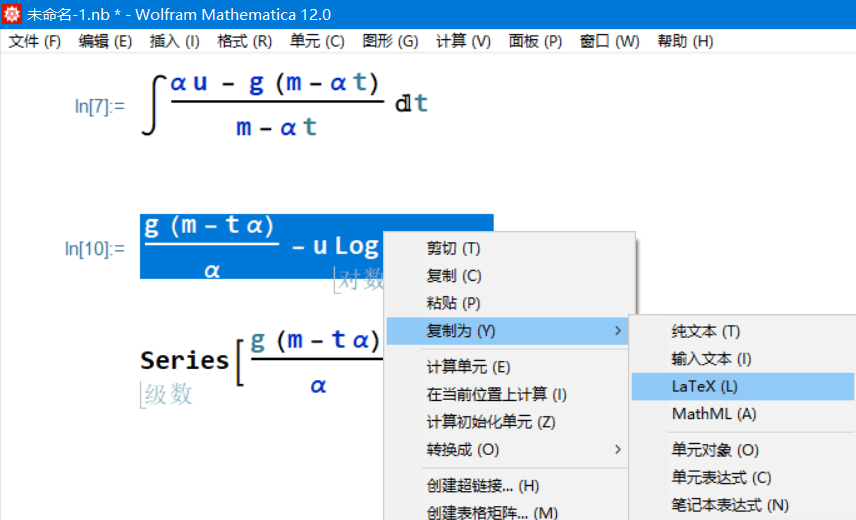
\includegraphics[width=0.8\textwidth]{figures//lll.png}
    \caption{从MMA中复制结果}\label{fig:show}
\end{figure}
\begin{equation}
    \frac{g \big(m(0)-\alpha  t\big)}{\alpha }-u \log \big(m(0)-\alpha  t\big) + \text{constant}
\end{equation}
考虑到第一项(g的一阶项)相比第二项很小,可以忽略。再带入初始条件
\begin{equation}
    v(0) = 0
\end{equation}
可以得到问题的解为
\begin{equation}
    u\Big(\ln m - \ln (m - \alpha t)\Big) =  u\ln \frac{m}{m - \alpha t}
\end{equation}

考虑到已知3(\ref{tab:bibi}), 可以得到火箭的最终速度不会大于$6.6\text{km/h}$小于宇宙第一速度。因此一级火箭不可行。
\subsection{问题二}
暂时忽略
\subsection{问题三}
暂时忽略
\section{模型的检验}\label{sec:6}

\section{模型的评价及推广}\label{sec:7}

\begin{thebibliography}{99}
  \bibitem{ref1}Tsiolkovsky K E. Cosmic Philosophy. Strelbytskyy Multimedia Publishing, 2020.
\end{thebibliography}

\begin{appendixx}
  \section{问题一的 Mathematica 代码}\label{p}
\begin{mma}
\[Integral](\[Alpha] u - g (m - \[Alpha] t))/(
  m - \[Alpha] t) \[DifferentialD]t
Series[(g (m-t \[Alpha]))/\[Alpha]-u Log[m-t \[Alpha]],{g, 0, 5}]

\end{mma}
\end{appendixx}
\end{document}